\chapter{Modellierung}\label{chap2}

\section{Nagel-Schreckenberg-Modell}
Bei der Modellierung des Straßenverkehrs gibt es verschiedene Ansätze. Je nachdem welche Fragen mit dem Modell beantwortet werden sollen, bzw. worauf man bei einem Modell Wert legt, fällt die Wahl des Modells aus. Bei der makroskopischen Simulation eines Verkehrsflussproblems wird der Straßenverkehr global betrachtet als fließende Bewegung, die hinsichtlich kollektiver Größen ausgewertet wird. Die Analyse des Modells erfolgt mithilfe von Geschwindigkeit und Dichte des Flusses. Möchte man die einzelnen Fahrzeuge betrachten und dabei die Anzahl pro Zeiteinheit oder die Dichte pro Strecke auswerten, so bietet sich der mikroskopische Simulationsansatz an, welcher auch bei der Simulation der Kreuzung verwendet wurde. \\
\\
Die Grundlage bei der mikroskopischen Simulation des Verkehrsflusses bildet das sogenannte Nagel-Schreckenberg-Modell. Dieses wurde nach Kai Nagel und Michael Schreckenberg benannt, die das Verkehrsmodell mithilfe der Theorie der zellulären Automaten entwickelt haben, siehe \cite{article:NaSch}. \\
\\
%Zelluläre Automaten
Ein zellulärer Automat ist ein sehr anschauliches Modell, das die Entwicklung von Zellen abhängig von deren eigenen Zustand und dem Zustand der Nachbarzellen beschreibt. Es besteht aus folgenden Komponenten, vergleiche Seite 181 in \cite{book:bungartz}: 
\begin{itemize}
 	  \item Zellraum\\
      		Diskreter Raum mit Zellen der gleichen Geometrie.
      \item Zustandsraum\\
      		Menge der möglichen Zustände der Zellen.
      \item Nachbarschaftsbeziehung\\
      		Nur die Zellen in der Nachbarschaft werden zur Kenntnis 				genommen.
      \item Diskrete Zeit \\
      		Änderung des Zustands einer Zelle in \( \delta \)t						Zeitschritten.
      \item Lokale Übergangsfunktion\\
      		Beschreibung der Veränderung des Zellzustands.
\end{itemize}
Es gibt viele verschiedene zelluläre Automaten mit unterschiedlichen Dimensionen. Zweidimensionale zelluläre Automaten kann man sich wie ein Gitter vorstellen, was in der folgenden Abbildung gut ersichtlich ist: \\
\begin{figure}[h]
\centering
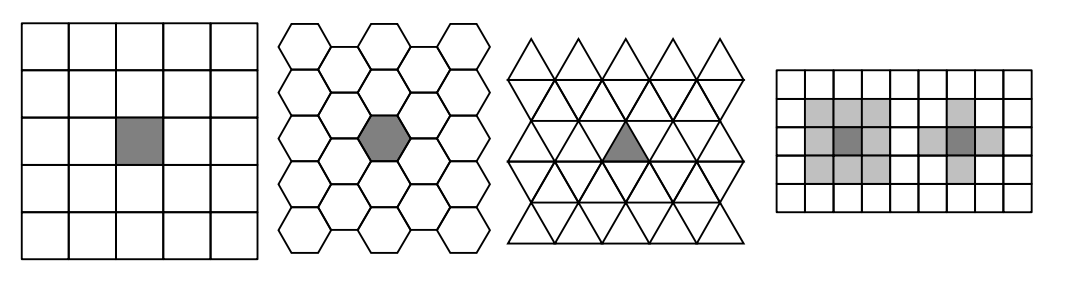
\includegraphics[width=10cm]{2_ZA_Beispiel.png}
\caption[Zweidimensionale zelluläre Automaten]{Beispiele zweidimensionale zelluläre Automaten, Quelle \cite{book:bungartz}, S. 181.}
\end{figure}

\hspace{-0.6cm} Was hat nun dieses Konzept mit Verkehrsproblemen bzw. -planung zu tun? Um das zu beantworten, kann man zunächst den einfachsten Fall betrachten: Einen einspurigen Straßenabschnitt. Weiterhin nehmen wir an, dass das System abgeschlossen ist. Das bedeutet, dass jedes Auto, welches am einen Ende der Fahrbahn hinaus fährt, beim anderen Ende wieder hinein fährt. Außerdem fahren alle Fahrzeuge in die gleiche Richtung. 
\\ \\
Unterteilen wir nun diesen Straßenabschnitt in mehrere Zellen, erhalten wir unseren Zellraum. Eine Zelle stellt also einen Teilabschnitt des gesamten Straßenabschnittes da. Die Größe der Zellen richtet sich beispielsweise nach dem Platz, den ein Auto mit Abstand zum Fahrzeug vor ihm minimal benötigt. 
\\ \\
Der Zustandsraum umfasst die Geschwindigkeiten der Fahrzeuge, wobei diese in Zellen pro Zeitschritt angezeigt wird. Dadurch ist auch gleichzeitig vorgegeben, wie weit ein Fahrzeug vorausschauen muss, um nicht mit anderen Autos zu kollidieren. 
\\ \\
Die Bestimmung der diskreten Zeitschritte erfolgt anhand von Verkehrsdaten. Dabei wird zum einen die Größe der Zellen benötigt. Zum anderen eine realistische Maximalgeschwindigkeit, beispielsweise die Geschwindigkeitsbegrenzung in Deutschland von 50 innerorts oder 100 auf Landstraßen. 
\\ \\
Die Übergangsfunktion muss nun noch vorgeben, wie sich die Geschwindigkeit eines Fahrzeugs von einem Zeitschritt auf den anderen verändert. Dabei ist im Modell des zellulären Automaten das Beschleunigen, Bremsen und Bewegen berücksichtigt, nicht aber die Trödelwahrscheinlichkeit. Diese kommt erst im Nagel-Schreckenberg-Algorithmus hinzu. 
\\ \\
Beim Nagel-Schreckenberg-Algorithmus wird jedes Fahrzeug nach einem Zeitschritt hinsichtlich seiner Geschwindigkeit neu betrachtet. Da unser Ziel ist, Staus zu vermeiden und gleichzeitig eine möglichst schnelle Fortbewegung zu erreichen, wird angenommen, dass jedes Fahrzeug genau die ihm mögliche Geschwindigkeit nutzt. Die Geschwindigkeit eines Fahrzeugs hängt also von der Anzahl der Zellen $d(i,j)$, die zwischen dem betrachteten Auto $i$ und dem vorher fahrenden Auto $j=i+1$ liegen und natürlich auch von der Maximalgeschwindigkeit \( v_{max} \) ab. Um das Modell noch realistischer zu machen, haben Schreckenberg und Nagel den Trödelfaktor eingefügt. Dieser bezieht ein, dass Fahrer möglicherweise zu stark abbremsen, zu langsam beschleunigen oder einfach trotz freier Fahrt konstante Geschwindigkeit halten. Diese Wahrscheinlichkeit wird mit $p$ bezeichnet.\\ 


\begin{algorithm}[H]\label{nagelschreckenberg_algo}
 %\SetLine % For v3.9
 %\SetAlgoLined % For previous releases [?]
 \KwData{ \\
   \(v_{i}, v_{max}, d(i,j), p \) 
 }
 \KwResult{ \\
    Update für Fahrzeug $i$
 }

 %initialization\;
 \For{ \(i \in \{1, \cdots, n\}\) }{
   Beschleunigen: \(v_{i} := min\{ v_{i}+1,v_{max}\} \);
   \\Bremsen: \(v_{i} := d(i,i+1), \text{ falls } v_{i} > d(i,i+1) \);
   \\Trödeln: \(v_{i} := max\{(v_{i}-1, 0 \}  \text{ mit } p < 1 \);
   \\Bewegen: Fahrzeug $i$ um \(v_{i}\) Zellen vorwärts bewegen;
 }
 
 \caption{Nagel-Schreckenberg-Algorithmus}
 \label{algo:nagelsberg}
\end{algorithm}



\section{Erweitertes Model für Kreuzungen} \label{sec:erwmodel}
Für die Modellierung einer Kreuzung benötigt man noch einige zusätzliche Annahmen. Unser Ziel ist es zwar mit einem Model die Realität möglichst gut abzubilden, doch muss dies im Verhältnis zur Komplexität des Models stehen. Um ein Modell und dessen Ergebnisse verstehen zu können, müssen Bedingungen hinzugefügt werden, die nicht immer identisch mit der Realität sind. Zudem machen manche Anforderungen die Simulation in einer annehmbaren Zeit überhaupt erst möglich. 
\\ \\
Zunächst betrachten wir die Straße an sich. Es handelt sich um zwei einspurige Ringstraßen, welche eine Zelle gemeinsam haben. Diese Zelle ist der Kreuzungspunkt der Straßen. Bildlich beschrieben kann man sich die Straßen auch bei der Modellierung als Kreuz vorstellen. Die Autos der einen Ringstraße können nur von links nach rechts fahren, die der anderen Straße nur von unten nach oben. Den Fahrzeugen ist es nicht möglich rückwärts oder nebeneinander zu fahren. Dadurch werden auch Überholvorgänge nicht abgebildet. Zudem wird der Zellraum als abgeschlossenes System betrachtet. Ein Verlassen der Straßen ist also nicht möglich. Fahrzeuge, die sich in der obersten Zelle bzw. in der Zelle ganz rechts befinden, setzen ihren Weg in der untersten Zelle bzw. in der Zelle ganz links fort. 
\\ \\
Nun müssen noch Regelungen für die Kreuzungszelle gefunden werden. Dabei werden drei Kreuzungstypen unterschieden \cite{book:bungartz}:
\begin{itemize}
	\item ungeregelte Kreuzung
      \item Kreisverkehr
      \item Kreuzungen mit geregelter Vorfahrt
\end{itemize}
Bei dem vorliegenden Model handelt es sich um eine ungeregelte Kreuzung. Es gilt also die Regel \glqq Rechts-vor-Links\grqq. Es gibt recht einfache Modelle, die die Regelung einer ungeregelten Kreuzung angeben, wie beispielsweise das Vier-Phasen-Modell, vergleiche Seite 198f. in \cite{book:bungartz}. Dieses verhindert auch das Auftreten von Deadlocks, welche entstehen können, wenn von allen vier Seiten gleichzeitig Fahrzeuge auf die Kreuzung zufahren. Da die Straßen in unserem Model jedoch nur einspurig sind, ergibt sich daraus eine einfache Regelung für die Vorfahrt: Die Fahrzeuge, die auf der vertikalen Straße fahren, haben immer Vorfahrt. 
\\ \\
Nun haben wir eine Regelung der Vorfahrt. Wie steht es allerdings mit der Geschwindigkeit auf und vor der Kreuzung? Betrachtet man die Realität, müssen Autos vor einer Kreuzung abbremsen, um nach vorfahrtsberechtigten Fahrzeugen Ausschau zu halten. Deshalb wurde in unserem Modell angenommen, dass jedes Fahrzeug vor der Kreuzungszelle auf die Maximalgeschwindigkeit von 1 Zelle pro Zeitschritt bremsen muss. Erst danach kann wieder beschleunigt werden, falls die Kreuzung frei ist. 

\begin{flushright}
Autor: Hannah Dusch
\end{flushright}
